\documentclass[../sparc.tex]{subfiles}
\graphicspath{{\subfix{../images/}}}
\begin{document}

%%%%%%%%%%%%%%%%%%%%%%%%%%%%%%%%%%%%%%%%%%%%%%%%%%%%%%%%%%%%%%%%%%%%%%%%%%%%%%%%
\section{Speaker connection}

There are several kinds of speakers that we can find.  For example, there are
``regular'' speakers where a membrane vibrates under the influence of a magnetic
field, generating acoustic waves in the air that we can hear as the sound.  Also
there are piezoelectric speakers where the acoustic waves are produced by the
reverse piezoelectric effect -- a mechanical deformation of a piezoelectric
material under an electric field. \footnote{See the ``Piezoelectric speaker''
article in the Wikipedia.}

The circuit for a regular speaker and a piezoelectric speaker is similar; for
the our tasks even simple piezoelectric speaker ``for Arduino'' is good enough.
Or we can use s simple beeper from a PC system board.

The schematic for the speaker connection is shown on the
fig. \ref{fig:sound-fig-2}.

\begin{figure}[h]
  \centering
  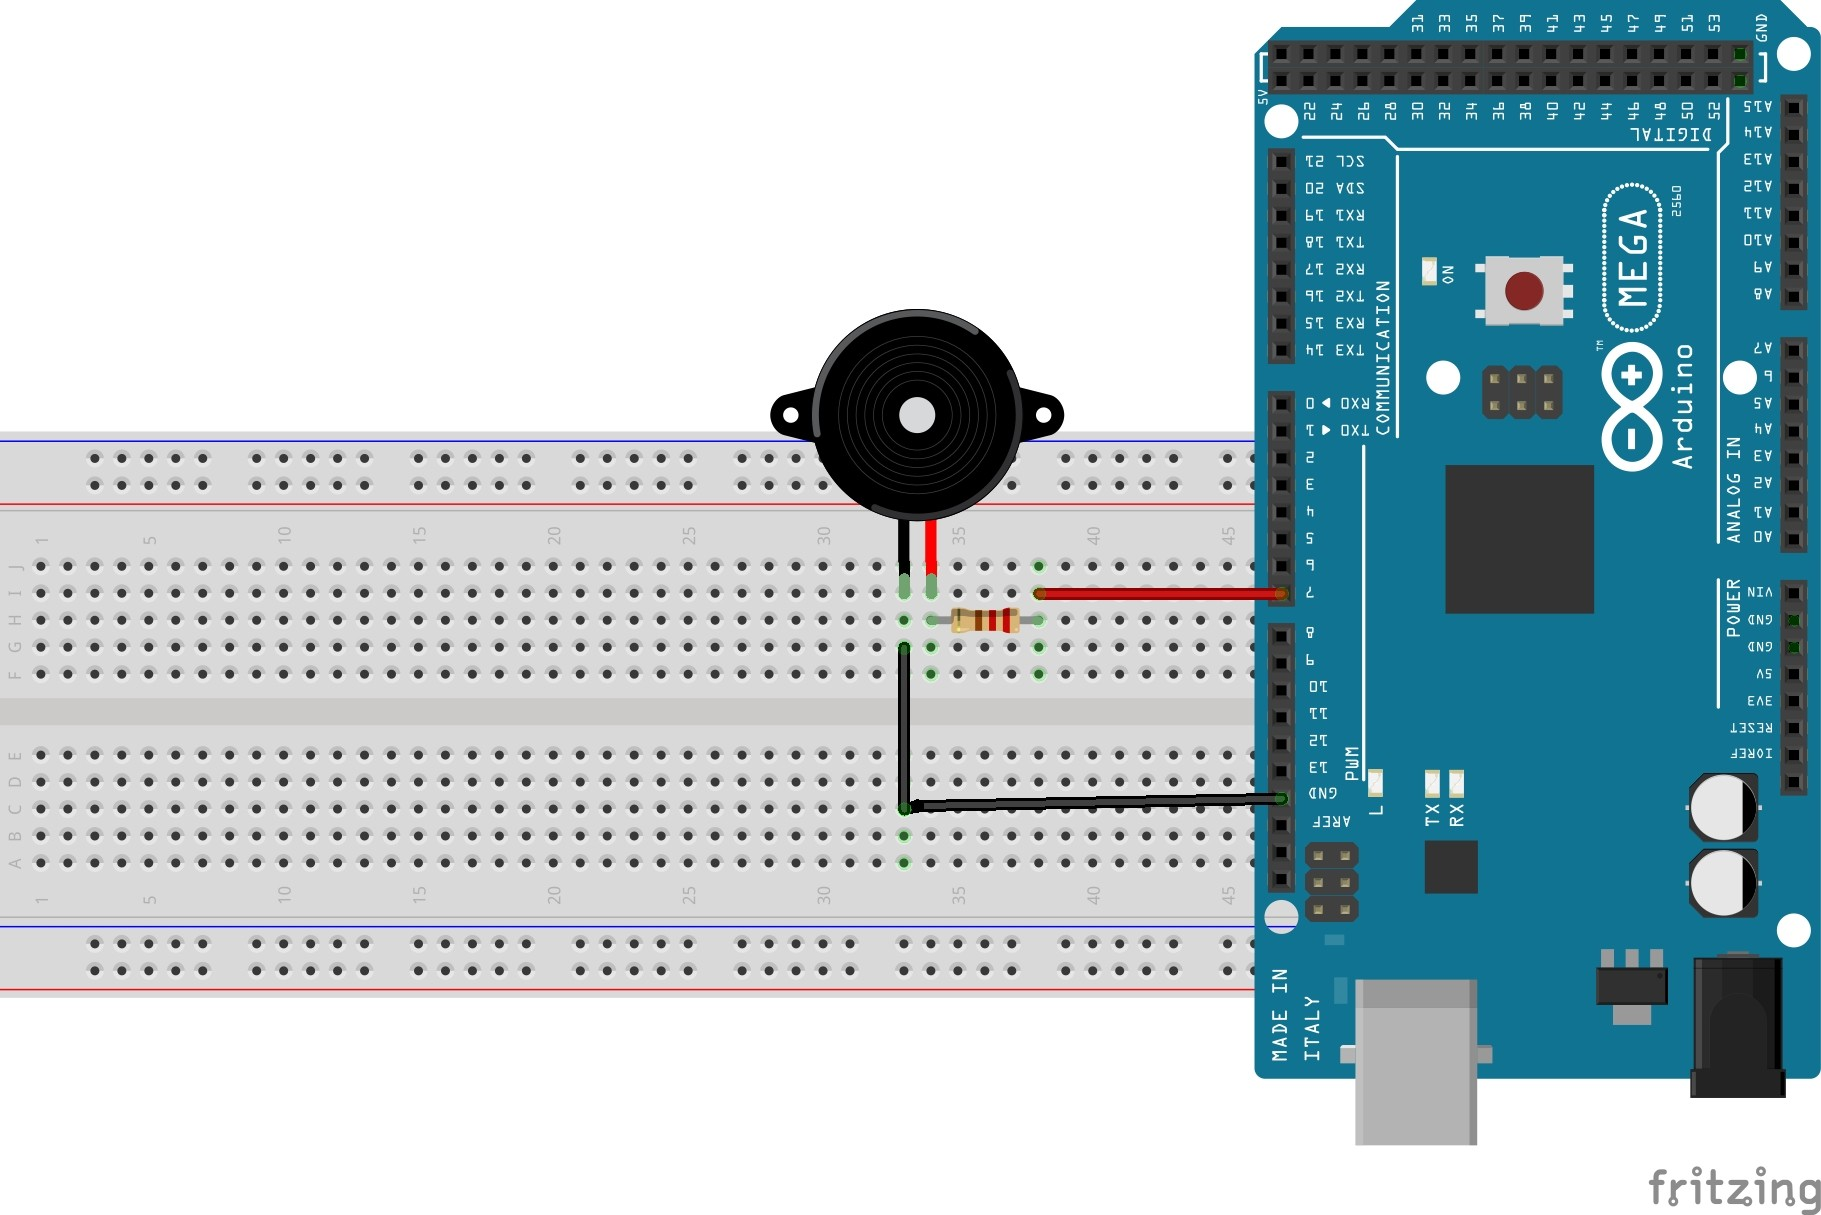
\includegraphics[width=10cm]{sound-fig-2}
  \caption{Connection of a speaker to the Arduino Mega 2560.}
  \label{fig:sound-fig-2}
\end{figure}

Let's build this circuit on a breadboard and upload our program for sound
generation to the Arduino.  Don't forget to configure a digital port for the
speaker in \texttt{OUTPUT} mode and add a call to our \texttt{play\_tone}
procedure in the \texttt{loop}.

For the convenience we will specify our port for the speaker as the
\texttt{SPEAKER\_PIN} constant at the top of our program (before the
\texttt{setup} procedure.)

Now we can generate a simple sound with the specified frequency.  But if we want
to generate something more interesting (a melody, for example) we have to use
sounds from the musical range.  In this case we have to get to know at least
some basics of the musical theory.

\subsection{Exercises}
\begin{enumerate}
\item Generate a sound with the frequency of 261.63 Hz.
\item Try to make the sound switch between 261.63 Hz and 349.23 Hz once a
  second.
\item Modify your program in such a way that to allow to change the sound
  frequency with a potentiometer.
\item Allow to switch the sound on and off by pressing a button connected to an
  Arduino.
\end{enumerate}

\end{document}
